\documentclass[11pt]{article}
\usepackage[spanish,es-noshorthands,es-tabla]{babel}
\usepackage[margin=2.4cm]{geometry}
\usepackage{amsmath,amssymb}
\usepackage{graphicx}
\usepackage{booktabs}
\usepackage{float}
\usepackage{caption}
\usepackage{enumitem}
\usepackage[hidelinks]{hyperref}

\graphicspath{{../figuras/}}
\newcommand{\tabla}[1]{\input{../tablas/#1.tex}}
\setlength{\parskip}{4pt}

\title{Análisis y Ciencia de Datos\\Tarea 3: Introducción a Series de Tiempo}
\author{Didvin Nohel Estrada Pineda \\ Carné 14092 \\ Ingeniería en Sistemas \\ Facultad de Ingeniería, Universidad del Istmo de Guatemala}
\date{25 de octubre de 2026}

\begin{document}
\maketitle

\noindent Todo el código está en \texttt{src/} y se corre con \texttt{python src/main.py} a partir del archivo \texttt{Online Retail.xlsx} original. Las tablas salen en \texttt{tablas/} y las figuras en \texttt{figuras/}. Las semillas usadas son: 14092 (+ número de escenario) en la Parte~0, las semillas 0 a 9 para la validación cruzada de la Parte~5 y 2026 en la Parte~6.

%======================================================================
\section{Parte 0: Procesos simulados}

\subsection*{0.1 A mano}
Sea $Y_t = c + \phi Y_{t-1} + \varepsilon_t$ con $|\phi|<1$ estacionario, así que $E[Y_t]=E[Y_{t-1}]=\mu$ y $\operatorname{Var}(Y_t)=\operatorname{Var}(Y_{t-1})=\gamma_0$.

\textbf{Media.} Tomando esperanza: $\mu = c + \phi\mu + 0$, entonces $\mu(1-\phi)=c$ y
\[ E[Y_t] = \frac{c}{1-\phi}. \]

\textbf{Varianza.} Como $\varepsilon_t$ es independiente de $Y_{t-1}$ (que solo depende de choques pasados), la covarianza entre ellos es cero:
\[ \gamma_0 = \operatorname{Var}(\phi Y_{t-1} + \varepsilon_t) = \phi^2\gamma_0 + \sigma^2 \quad\Rightarrow\quad \operatorname{Var}(Y_t)=\frac{\sigma^2}{1-\phi^2}. \]

\textbf{Autocorrelación.} Para $k\ge 1$, usando otra vez que $\varepsilon_t$ no está correlacionado con $Y_{t-k}$:
\[ \gamma_k = \operatorname{Cov}(Y_t, Y_{t-k}) = \operatorname{Cov}(c+\phi Y_{t-1}+\varepsilon_t,\, Y_{t-k}) = \phi\,\gamma_{k-1}. \]
Aplicando la recursión $k$ veces, $\gamma_k = \phi^k\gamma_0$, así que $\rho_k=\gamma_k/\gamma_0=\phi^k$.

\textbf{Caminata aleatoria.} Con $\phi=1$, $c=0$ y $Y_0=0$, al sustituir hacia atrás $Y_t = \sum_{j=1}^{t}\varepsilon_j$. Los choques son independientes, entonces
\[ \operatorname{Var}(Y_t)=\sum_{j=1}^{t}\operatorname{Var}(\varepsilon_j)=t\sigma^2. \]
La varianza depende de $t$ (crece sin límite), y la estacionariedad débil pide varianza constante, así que no es estacionaria. También se ve en la fórmula $\sigma^2/(1-\phi^2)$, que explota cuando $\phi\to1$.

\subsection*{0.2 Simulación}
La función \texttt{simular\_ar1} (en \texttt{parte0\_simulacion.py}) arranca en $Y_0=0$, simula 500 pasos y descarta los primeros 200. Para $|\phi|<1$ esto sirve porque el efecto del valor inicial decae como $\phi^t$. Para $\phi=1$ no lo logra: la caminata nunca olvida, $Y_{200+s} = Y_{200} + \sum \varepsilon$, y la varianza sigue creciendo. Aun así no afecta a $r_k$, porque $r_k$ resta la media muestral: sumarle una constante ($Y_{200}$) a toda la serie no cambia ni el numerador ni el denominador.

La Figura~\ref{fig:p0real} muestra una realización de cada $\phi$. Con $\phi=0$ la serie cruza la media todo el tiempo; con $\phi=0.9$ se aleja y tarda en regresar; con $\phi=1$ deambula sin regresar a ningún nivel.

\begin{figure}[H]\centering
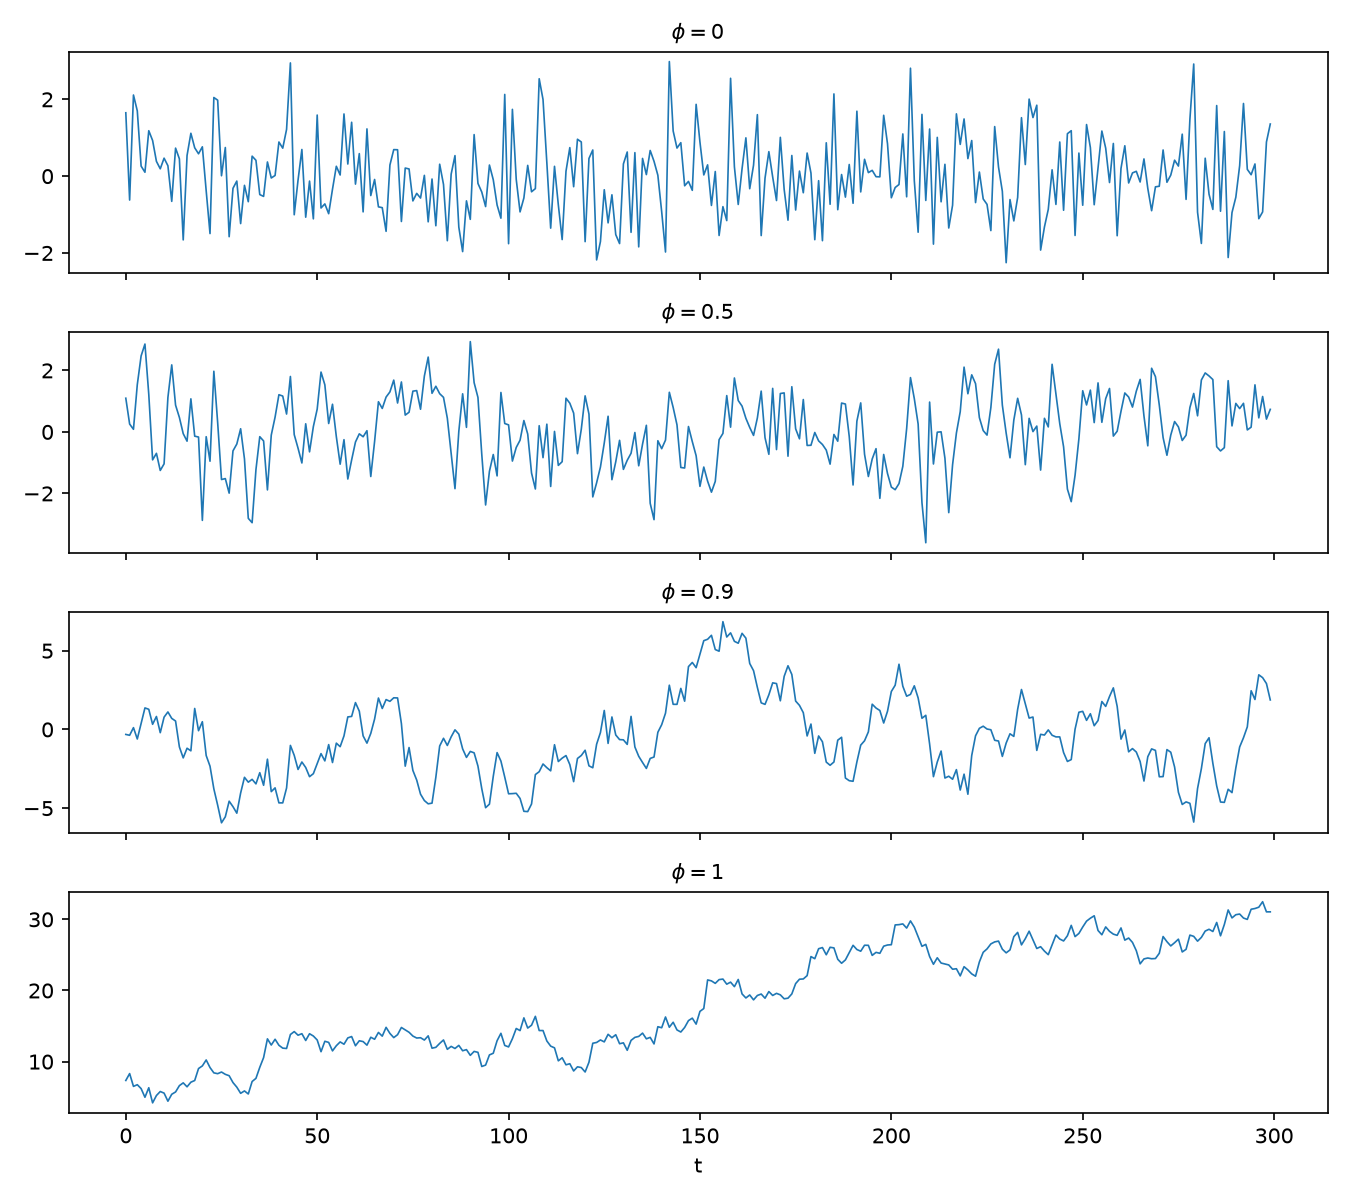
\includegraphics[width=0.85\textwidth]{p0_realizaciones.png}
\caption{Una realización de 300 pasos para cada $\phi$.}\label{fig:p0real}
\end{figure}

La Tabla~\ref{tab:p0ar1} resume las 5\,000 réplicas por escenario, con el error estándar de cada promedio (desviación estándar entre réplicas sobre $\sqrt{5000}$).

\begin{table}[H]\centering\small
\caption{AR(1), 5\,000 réplicas de $n=300$. ``rechazo r1'' es la fracción de réplicas con $|r_1|>1.96/\sqrt{n}$.}\label{tab:p0ar1}
\resizebox{\textwidth}{!}{\tabla{p0_tabla_ar1}}
\end{table}

\subsection*{0.3 Interpretación}
Con $\phi=0$ la tasa de rechazo es 5.14\,\% (e.e.\ 0.31\,\%), que es lo esperado: la banda $\pm1.96/\sqrt n$ es un intervalo del 95\,\% bajo ruido blanco, así que en el 5\,\% de los casos se sale por azar. El promedio de $r_1$ es $-0.004$, muy cerca del sesgo teórico $-1/n\approx-0.0033$ que aparece por estimar la media.

Para la caminata aleatoria, el promedio de $r_5$ es 0.882 y no 1. La ``teoría'' $\phi^5=1$ no aplica porque la caminata no es estacionaria y $\rho_k$ no está definida; además $r_k$ calcula desviaciones respecto a una media muestral que no representa a ningún nivel de la serie, lo que la empuja hacia abajo. Incluso el $r_1$ promedio queda en 0.976.

El estimado OLS de $\phi$ tiene un sesgo hacia abajo que crece con $\phi$: $-0.009$ para $\phi=0.5$, $-0.013$ para $0.9$ y $-0.018$ para $1$. Estos valores coinciden con la aproximación clásica $-(1+3\phi)/n$ (por ejemplo $-3.7/300=-0.0123$ para $\phi=0.9$). Es un sesgo de orden $1/n$, por lo que el estimador es consistente: con más datos el sesgo desaparece. Con $\phi=1$ el sesgo es el mayor, aunque el estimador converge aun más rápido (orden $1/n$ en vez de $1/\sqrt n$).

\subsection*{0.4 Las dos razones para reprobar}

\begin{table}[H]\centering\small
\caption{Procesos sin memoria con media que cambia (5\,000 réplicas).}\label{tab:p0sm}
\tabla{p0_tabla_sin_memoria}
\end{table}

\begin{figure}[H]\centering
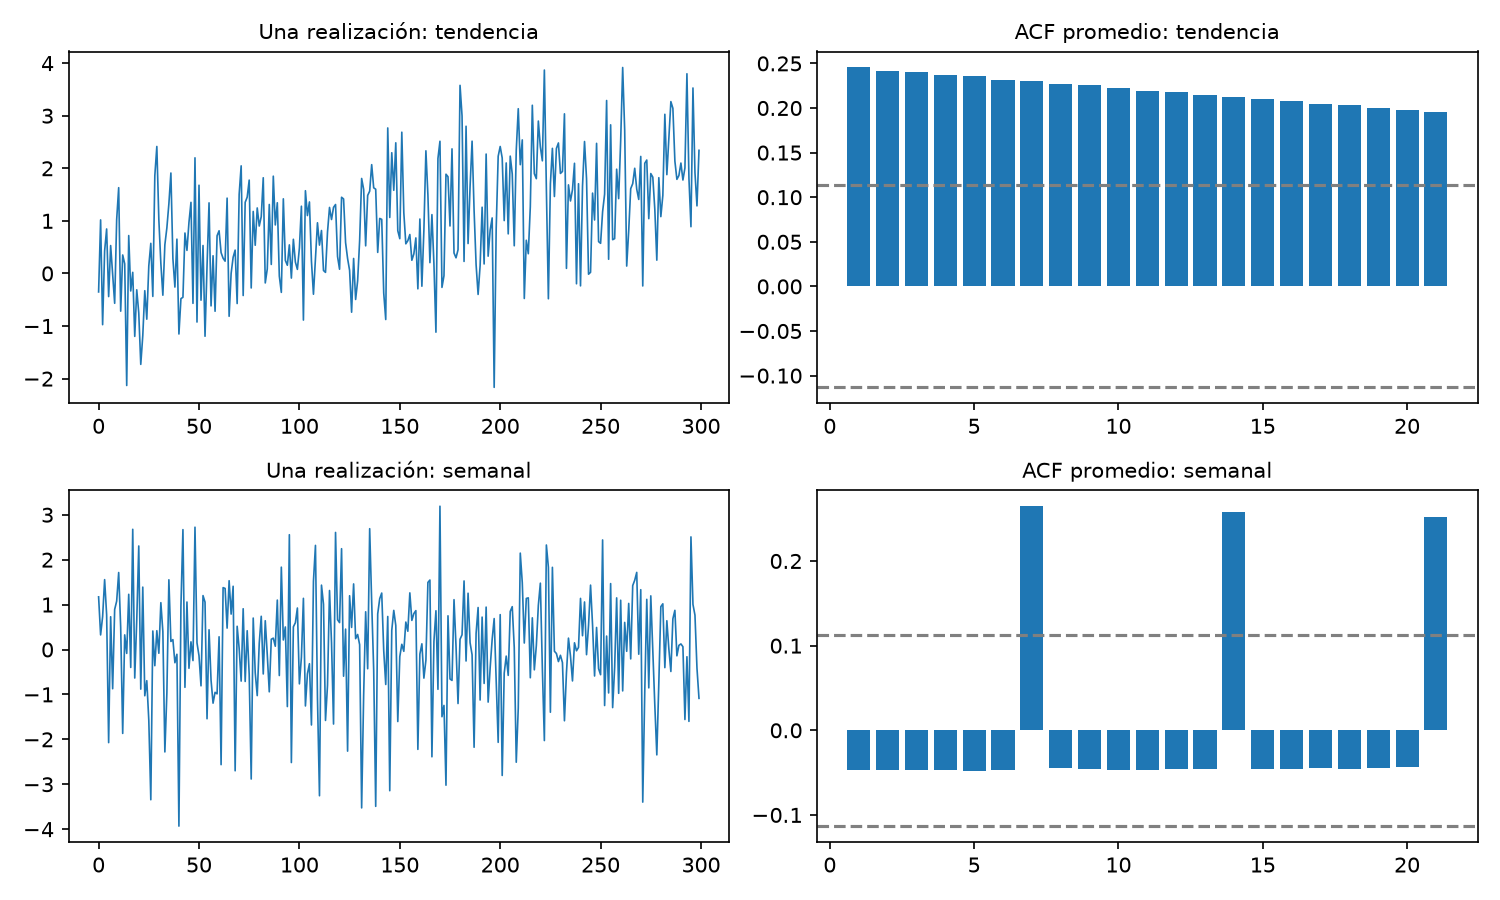
\includegraphics[width=0.9\textwidth]{p0_sin_memoria.png}
\caption{Una realización y la ACF promedio de cada proceso sin memoria.}\label{fig:p0sm}
\end{figure}

La tendencia reprueba la prueba de retardo 1 en el 98.6\,\% de las réplicas aunque no tiene ninguna memoria: los datos del final están todos arriba de $\bar y$ y los del principio todos abajo, así que los vecinos ``se parecen'' y $r_1\approx 0.25$. Su ACF baja despacio (Figura~\ref{fig:p0sm}), justo la pista visual de la razón (2).

El patrón semanal \emph{pasa} la prueba de retardo 1 en casi el 90\,\% de los casos (rechazo de 10.7\,\%), aunque tiene una estructura fuertísima: $r_7=0.265$. La prueba solo mira el rezago 1, y el patrón vive en el rezago 7. Eso es lo mismo que pasaba con RANDU en la Tarea 2: pasaba las pruebas que miraban pares consecutivos, pero tenía una estructura muy marcada (las ternas caían en 15 planos) que solo se ve mirando en la dimensión o el rezago correcto. Pasar una prueba nunca demuestra independencia; solo dice que esa prueba no encontró la dependencia.

\subsection*{0.5 La prueba que sí ve}

\begin{table}[H]\centering\small
\caption{Rechazo de Ljung--Box con $m=10$ al 5\,\%. La última columna compara los valores $p$ propios con \texttt{acorr\_ljungbox} en 50 réplicas.}
\tabla{p0_tabla_ljungbox}
\end{table}

Con ruido blanco Ljung--Box rechaza el 5.6\,\%, que es el nivel nominal. Para la tendencia rechaza siempre. El cambio importante es el patrón semanal: pasa de 10.7\,\% de rechazo a 95.6\,\%. La diferencia es que $Q(10)$ junta los rezagos 1 a 10, que incluyen el 7, así que ve el patrón que la prueba de retardo 1 no veía. La implementación propia coincide con statsmodels hasta el error de redondeo.

%======================================================================
\section{Los datos}
\texttt{InvoiceNo}, \texttt{StockCode} y \texttt{CustomerID} se leen como texto porque: \texttt{InvoiceNo} tiene prefijos (\texttt{C}, \texttt{A}) que se perderían o darían error como número; \texttt{StockCode} mezcla dígitos y letras (\texttt{85123A}, \texttt{POST}) y como número se perderían los ceros o las letras; y \texttt{CustomerID}, como tiene faltantes, pandas lo lee como \texttt{float} (\texttt{17850.0}), lo que estorba al comparar o unir. Ninguno de los tres es una cantidad: son etiquetas.

%======================================================================
\section{Parte 1: Limpieza}

\subsection*{1.1 Conteos}
\begin{table}[H]\centering\small
\caption{Conteos del archivo original.}
\tabla{p1_conteos}
\end{table}
El 24.9\,\% de las filas no tiene \texttt{CustomerID}.

\subsection*{1.2 Casos}
\begin{table}[H]\centering\small
\caption{Filas y monto ($Q\times P$) de cada caso, medidos por separado sobre los datos crudos.}
\tabla{p1_casos}
\end{table}

\begin{enumerate}[label=(\alph*)]
\item \textbf{Duplicados exactos (5\,268).} Se van. Una fila idéntica en factura, producto, cantidad, precio, cliente y minuto es casi seguro un error de registro; si fuera una compra legítima del mismo artículo, el sistema la habría sumado en una sola línea.
\item \textbf{Facturas que no empiezan con dígito.} Las de prefijo \texttt{C} (9\,288) son cancelaciones: se quedan con su signo negativo para que resten el día en que ocurren. Las de prefijo \texttt{A} (3 filas) son ``Adjust bad debt'', ajustes contables de deuda incobrable que no son ventas: se van.
\item \textbf{Códigos que no son productos.} Los códigos que no empiezan con cinco dígitos se revisaron uno por uno (tabla \texttt{p1\_codigos\_no\_numericos}). Se van: \texttt{POST}, \texttt{DOT}, \texttt{C2} (envíos), \texttt{M}/\texttt{m} (Manual), \texttt{D} (descuento), \texttt{S} (muestras), \texttt{B} (ajuste de deuda), \texttt{BANK CHARGES}, \texttt{AMAZONFEE}, \texttt{CRUK} (comisiones) y los vales \texttt{gift\_0001\_*}, que son dinero prepagado y no mercadería. Se quedan los \texttt{DCGS*} (``GIRLS PARTY BAG'', ``BOXED GLASS ASHTRAY''...) y \texttt{PADS}, que sí son artículos con precio normal. El caso \texttt{M} tiene un detalle que se ve en 1.4: algunas ventas se anularon con una línea Manual en vez de una cancelación del producto. Para esos casos se agregó una regla que quita la venta y su anulación juntas.
\item \textbf{Precios cero o negativos.} Se van. Los 2\,515 con precio cero no generan venta y casi todos son notas internas (``check'', ``damages'', ``found''). Los 2 negativos son los ajustes de deuda \texttt{B}.
\item \textbf{Cantidades negativas sin \texttt{C} (1\,336).} Todas tienen precio 0 y descripciones como ``check'', ``damaged'', ``thrown away'' o ``sold as set on dotcom'': son ajustes de inventario, no devoluciones de clientes. Se van (no cambian el monto).
\item \textbf{Sin \texttt{CustomerID} (135\,080 filas, £1.45 millones).} Para la serie de ventas se quedan: la venta ocurrió aunque no sepamos quién compró, y quitarla bajaría el nivel de la serie una cuarta parte. Para la Parte 6 se quitan, porque ahí la unidad de análisis es el cliente (\texttt{limpiar(df, con\_cliente=True)}).
\end{enumerate}

\subsection*{1.3 Bitácora de limpieza}
\begin{table}[H]\centering\small
\caption{Bitácora en el orden en que se aplican las reglas. ``monto'' es la suma con signo y ``monto\_abs'' la suma de valores absolutos de lo eliminado.}
\tabla{p1_bitacora}
\end{table}
El orden importa: la cantidad negativa sin cancelación va antes que el precio cero, así que las 1\,336 filas de ajustes se cuentan en la regla 5 y la regla 6 solo ve las 1\,157 que quedan con precio 0. Los duplicados van primero para que los demás conteos sean de filas únicas, y la regla de anulaciones Manual va antes de quitar los códigos no producto (si no, la línea \texttt{M} desaparecería y la venta se quedaría sola). Quedan 531\,202 filas con una venta neta de £9.73 millones.

\subsection*{1.4 Las seis líneas más grandes}
\begin{table}[H]\centering\scriptsize
\caption{Las seis líneas con mayor $|Q\times P|$ antes de limpiar.}
\resizebox{\textwidth}{!}{\tabla{p1_top6}}
\end{table}
Son tres pares:
\begin{itemize}
\item \textbf{581483 / C581484}: el cliente 16446 pidió 80\,995 ``PAPER CRAFT, LITTLE BIRDIE'' (£168\,470) el 9 de diciembre a las 9:15 y se canceló 12 minutos después. Es claramente un error de digitación.
\item \textbf{541431 / C541433}: el cliente 12346 pidió 74\,215 frascos de cerámica (£77\,184) el 18 de enero y se canceló 16 minutos después. Ese cliente no volvió a comprar, y por eso aparece con $M=0$ en la Parte 6.
\item \textbf{556444 / C556445}: 60 canastas de picnic a £649.50 cada una (£38\,970), anuladas tres minutos después con una línea \texttt{M} Manual por el mismo monto. El precio unitario es absurdo para el artículo.
\end{itemize}
La limpieza no quita los dos primeros pares (son ventas y cancelaciones válidas), pero el neteo por día los resuelve: venta y cancelación caen el mismo día y se anulan. El tercero sí lo resuelve la limpieza con la regla de anulaciones Manual. Sin esa regla, la regla 4 quitaría la línea \texttt{M} y dejaría una venta fantasma de £38\,970 el 10 de junio que el neteo ya no podría compensar. Si en cambio dejáramos la línea \texttt{M}, el neteo diario la resolvería.

\subsection*{1.5 La función \texttt{limpiar}}
Está en \texttt{src/limpieza.py}. Recibe el DataFrame crudo, aplica las reglas en el orden de la bitácora, agrega la columna \texttt{Monto} y, si se le pasa una lista, va anotando la bitácora. Con \texttt{con\_cliente=True} también quita las filas sin \texttt{CustomerID}.

%======================================================================
\section{Parte 2: El calendario}

\subsection*{2.1 y 2.2}
Entre el 1 de diciembre de 2010 y el 9 de diciembre de 2011 hay 374 días calendario y hubo transacciones en 305. De los 69 días sin transacciones, 53 son sábados: la tienda no abre los sábados (no hay ni una sola transacción en sábado). Los otros 16 son:

\begin{table}[H]\centering\small
\caption{Días sin transacciones que no son sábado.}
\tabla{p2_dias_faltantes}
\end{table}

Son el cierre de fin de año (del 24 de diciembre al 3 de enero, que incluye los feriados sustitutos de Navidad, Boxing Day y Año Nuevo), la Semana Santa (Viernes Santo 22 de abril, Domingo de Pascua 24 y Lunes de Pascua 25), la boda real del 29 de abril de 2011 (el feriado que no se repite) y los tres bank holidays de lunes: 2 de mayo, 30 de mayo y 29 de agosto. Los móviles son los de Semana Santa: su fecha depende del calendario lunar y cambia hasta un mes de un año a otro, por eso son los más difíciles de modelar con datos diarios. Los de mayo y agosto también cambian de fecha, pero siempre caen en lunes de una semana fija del mes.

\begin{figure}[H]\centering
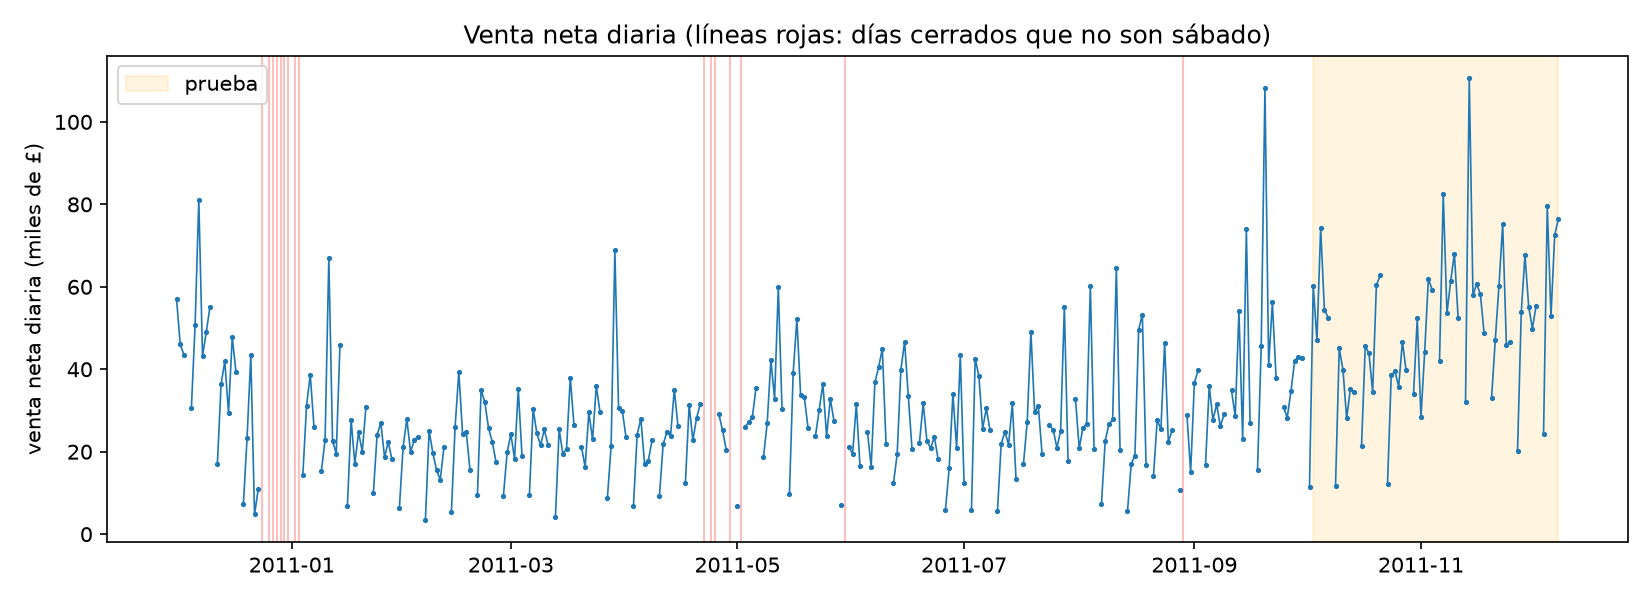
\includegraphics[width=\textwidth]{p2_serie_diaria.png}
\caption{Venta neta diaria. Las líneas rojas marcan días cerrados que no son sábado; la zona naranja es el periodo de prueba.}\label{fig:p2}
\end{figure}

\subsection*{2.3 ¿Cero o faltante?}
Depende del uso. Si queremos la venta total de diciembre, o la venta acumulada del año, el día cerrado es un \textbf{cero}: ese día entró £0 y sumarlo como cero da el total correcto. Si queremos modelar la venta de un día en que la tienda está abierta (pronosticar, medir el efecto del día de la semana o calcular la ACF), es un \textbf{faltante}: no hubo mercado ese día, y un cero se vería como un desplome de ventas que el modelo trataría de explicar.

\subsection*{2.4 El último día}
El 9 de diciembre está incompleto: la última transacción es a las 12:50, mientras que la mediana de la hora de la última transacción de cada día es las 17:00. Además, ese día está el pedido de 80\,995 unidades y su cancelación. Lo quitamos de la serie, porque una venta de medio día se vería como una caída que no ocurrió.

Con esto queda la serie con calendario completo, días cerrados como faltantes y sin el 9 de diciembre: 245 días abiertos en entrenamiento (hasta el 30 de septiembre) y 58 días abiertos en prueba (del 3 de octubre al 8 de diciembre).

%======================================================================
\section{Parte 3: Tendencia, estacionalidad y autocorrelación}

\subsection*{3.1 Tendencia}
\begin{figure}[H]\centering
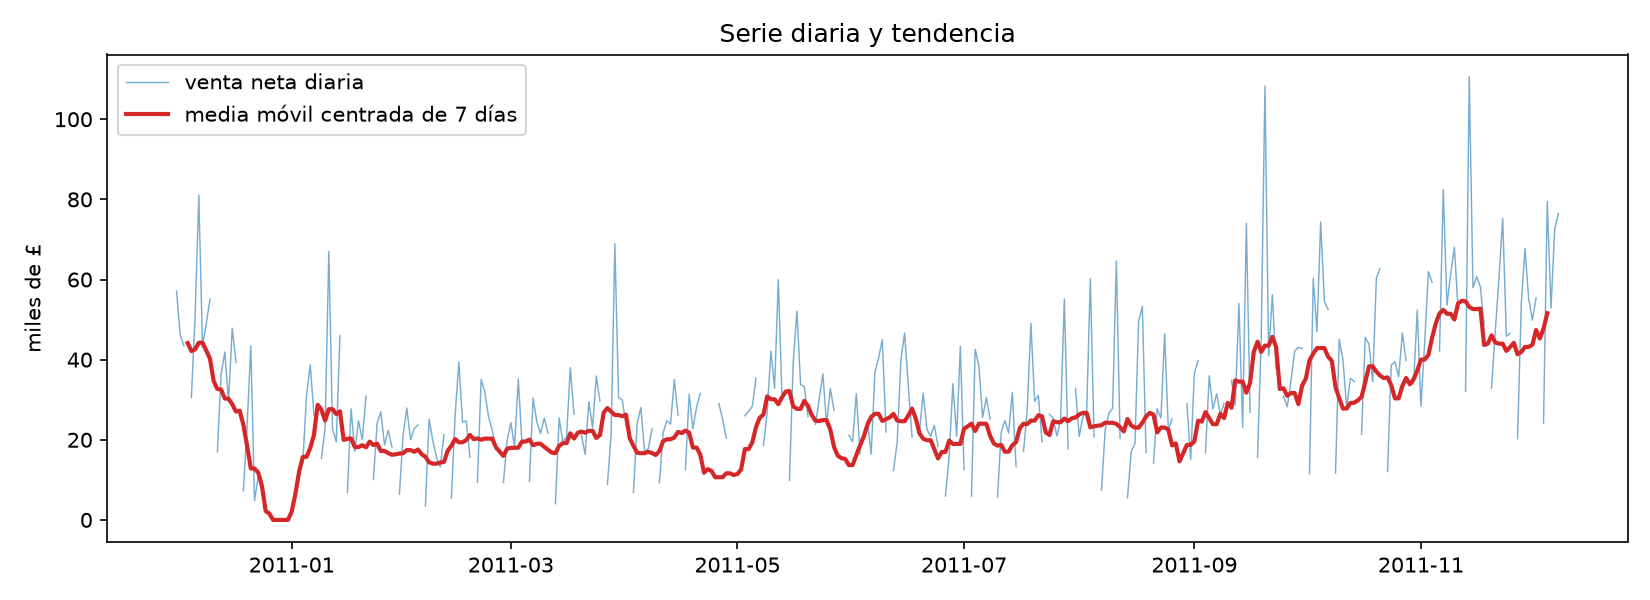
\includegraphics[width=\textwidth]{p3_tendencia.png}
\caption{Serie diaria (cerrados = 0) y su media móvil centrada de 7 días.}\label{fig:p3t}
\end{figure}

Se usa 7 porque el patrón se repite cada semana: una ventana de 7 días contiene exactamente un día de cada tipo, así que el efecto del día de la semana se cancela y solo queda el nivel. Con 5 la ventana tendría unos días de la semana dos veces y otros ninguna, y el promedio subiría o bajaría según dónde cae (seguiría teniendo patrón semanal). Con 30 se mezclarían semanas incompletas y se suavizaría tanto que se perdería cuándo empieza a subir la serie. Es centrada (de $t-3$ a $t+3$) para que no tenga rezago: una media móvil hacia atrás reacciona tarde y desplaza la tendencia unos días a la derecha.

La tendencia está más o menos plana entre £17\,000 y £24\,000 diarias de diciembre a agosto (con bajones en enero y abril por los cierres), y a partir de septiembre sube con fuerza: £32\,500 en septiembre, £35\,000 en octubre y £47\,000 en noviembre. Es la temporada navideña de una tienda de regalos que le vende a mayoristas, que compran con anticipación.

\subsection*{3.2 Estacionalidad}
\begin{table}[H]\centering\small
\caption{Índice estacional por día de la semana (promedio de $y_t/\text{MA}_t$ en los días abiertos del entrenamiento).}\label{tab:idx}
\tabla{p3_indices}
\end{table}

\begin{figure}[H]\centering
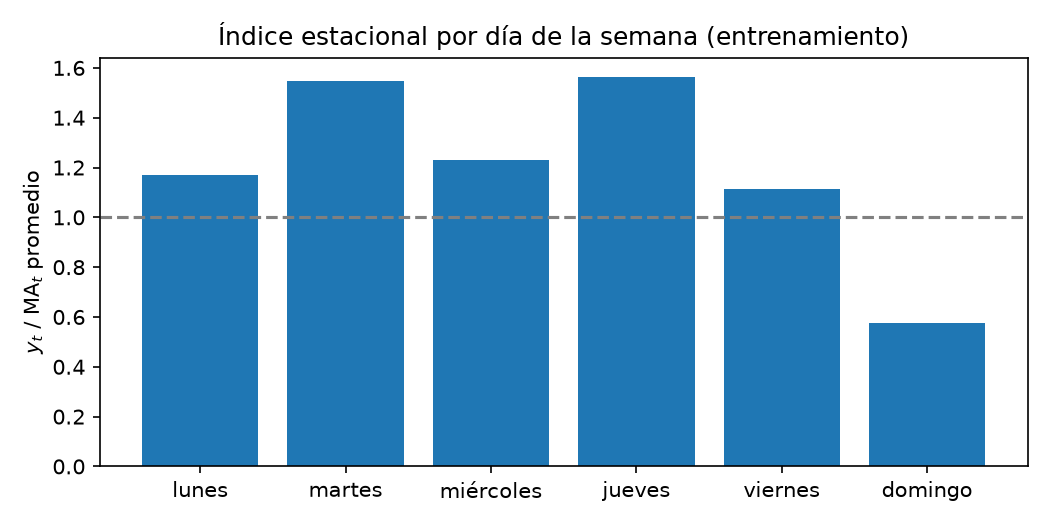
\includegraphics[width=0.6\textwidth]{p3_indices.png}
\caption{Índices estacionales.}
\end{figure}

Martes (1.55) y jueves (1.56) son los días que más venden, seguidos de miércoles y lunes; el domingo vende menos de la mitad que el martes (0.58). El promedio de los seis índices es 1.20 y no 1 porque la media móvil incluye los sábados con cero. La venta de la semana se reparte en seis días abiertos pero se divide entre siete, así que en un día abierto típico $y_t/\text{MA}_t\approx 7/6\approx1.17$. El resto de la diferencia viene de los feriados (que también entran como cero en la media móvil y suben los cocientes de su semana).

\subsection*{3.3 Autocorrelación}
\begin{figure}[H]\centering
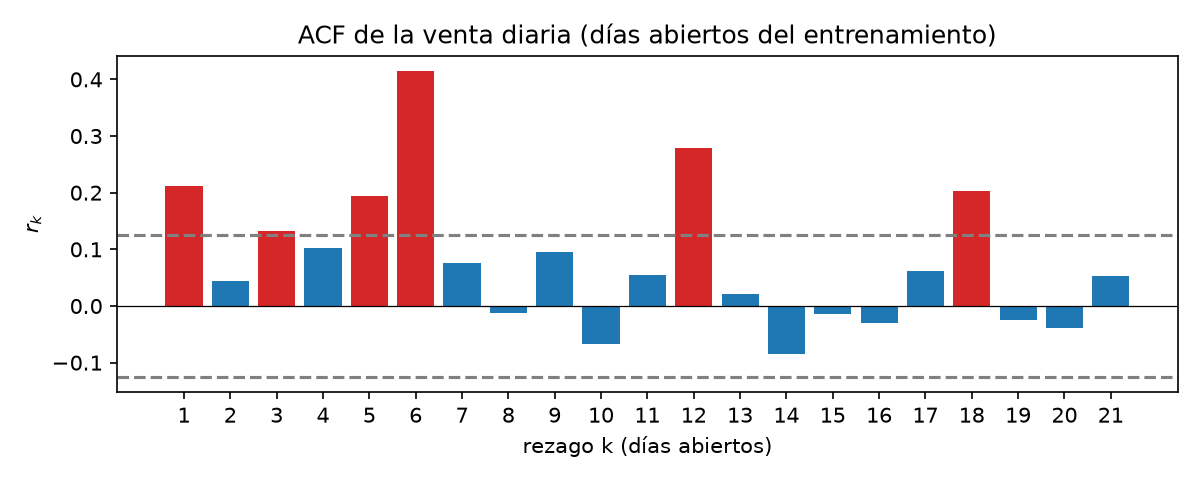
\includegraphics[width=0.8\textwidth]{p3_acf.png}
\caption{ACF de los 245 días abiertos del entrenamiento, con bandas $\pm1.96/\sqrt{245}=\pm0.125$. En rojo los rezagos que se salen.}\label{fig:p3acf}
\end{figure}

\begin{enumerate}[label=(\alph*)]
\item Se salen 6 de los 21 rezagos: 1, 3, 5, 6, 12 y 18. Con $r_1=0.212>0.125$ no pasa la prueba de retardo 1 de la Tarea 2. El pico está en $k=6$ ($r_6=0.414$), que son seis días abiertos, o sea siete días calendario: una semana (seis días abiertos más el sábado cerrado). Los rezagos 12 y 18 son dos y tres semanas. Ljung--Box lo confirma: $Q(6)=71.6$ y $Q(12)=97.6$, con valores $p$ de $10^{-13}$ y $10^{-15}$.

\begin{table}[H]\centering\small
\caption{Ljung--Box sobre la venta diaria (días abiertos del entrenamiento).}
\tabla{p3_ljungbox}
\end{table}

\item Con lo que vimos en la Parte 0, los picos en 6, 12 y 18 se parecen al proceso semanal: es una media que cambia con el día de la semana, no memoria. La ACF positiva en casi todos los rezagos que baja despacio se parece a la del proceso con tendencia, y también puede ser media no constante (el aumento de septiembre). Solo lo que quede después de quitar esas dos cosas es memoria de verdad; eso es lo que mide la Parte 4.
\end{enumerate}

%======================================================================
\section{Parte 4: Del AR(1) al SARIMA}

\subsection*{4.1 Quitar el día de la semana}
La regresión sin intercepto con seis indicadoras da como coeficientes la media de cada día: £27.2k (lunes), £35.2k (martes), £27.8k (miércoles), £35.4k (jueves), £26.3k (viernes) y £13.7k (domingo).

\begin{figure}[H]\centering
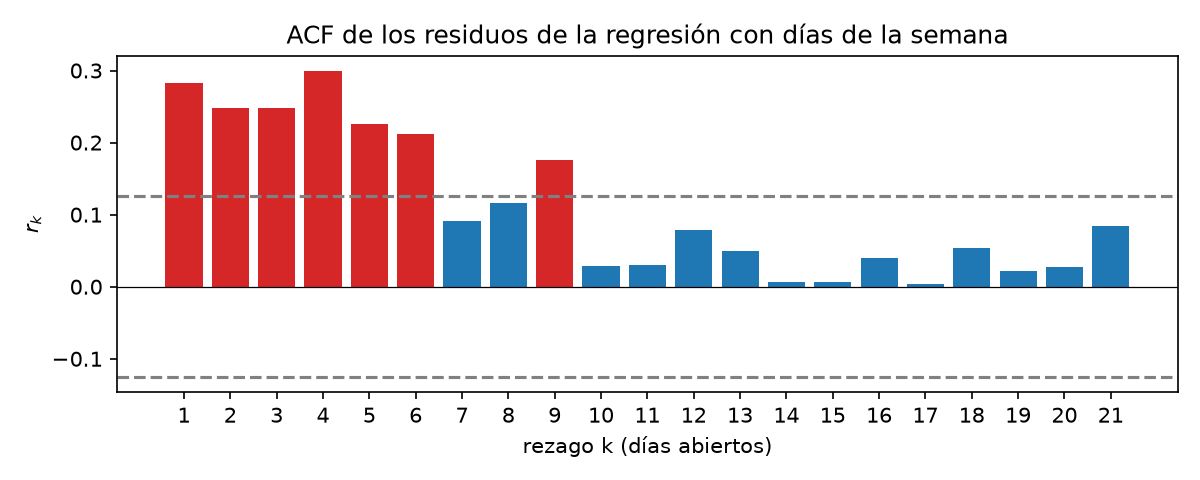
\includegraphics[width=0.8\textwidth]{p4_acf_dummies.png}
\caption{ACF de los residuos $e_t$ de la regresión con días de la semana.}\label{fig:p4d}
\end{figure}

Los picos semanales desaparecen ($r_6$ baja de 0.41 a 0.21 y $r_{12}$, $r_{18}$ quedan dentro de las bandas), pero ahora los rezagos 1 a 6 están todos entre 0.21 y 0.30 y bajan muy despacio. Eso no es como un AR(1): con $r_1=0.28$, un AR(1) tendría $r_6=0.28^6\approx0.0005$. Se parece mucho más a la ACF del proceso con tendencia de la Parte 0. A este modelo le falta la tendencia: las medias por día son constantes en todo el año y no ven que el nivel sube en otoño, así que 22 de los 26 residuos de septiembre quedan positivos.

\subsection*{4.2 AR(1) sobre los residuos}
El AR(1) estimado por OLS da $\hat\phi=0.285$ (y $\hat c\approx-101$, prácticamente cero). Los residuos $u_t$ todavía tienen rezagos fuera de las bandas en 4, 6 y 9 (Figura~\ref{fig:p4ar}). Ljung--Box con un grado de libertad menos: $Q(6)=24.3$ con 5 g.l.\ ($p=0.0002$) y $Q(12)=33.2$ con 11 g.l.\ ($p=0.0005$). No parecen ruido blanco: el AR(1) no alcanza, porque lo que encontramos en 4.1 no es memoria corta sino un nivel que se mueve, y un AR(1) estacionario con $\phi=0.28$ olvida en dos o tres días.

\begin{figure}[H]\centering
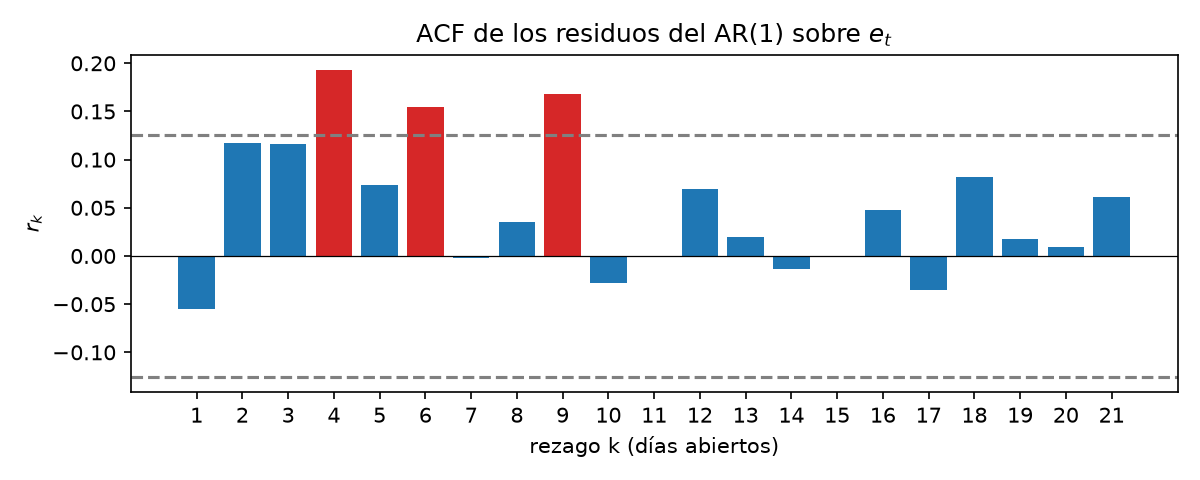
\includegraphics[width=0.8\textwidth]{p4_acf_ar1.png}
\caption{ACF de los residuos del AR(1) ajustado a $e_t$.}\label{fig:p4ar}
\end{figure}

\subsection*{4.3 SARIMA}
Se usa $s=6$ porque trabajamos con una fila por día abierto, y una semana tiene seis días abiertos; con $s=7$ estaríamos comparando, por ejemplo, un lunes con el martes de la semana anterior. La suposición se rompe con los feriados y los cierres: en una semana con un lunes feriado hay solo cinco filas, y a partir de ahí el rezago 6 ya no es el mismo día de la semana hasta que pasa la ventana. Pasa con Semana Santa, con los tres lunes feriados y con el cierre de fin de año.

Se usa el logaritmo porque la variación crece con el nivel: en noviembre las diferencias entre días son mucho más grandes que en febrero. FPP2 recomienda transformar cuando la variación aumenta con el nivel, y con el logaritmo un patrón multiplicativo (el martes vende 1.5 veces la tendencia) se vuelve aditivo, que es lo que suponen los SARIMA. Se puede usar porque la venta diaria mínima del entrenamiento es £3\,440 (no hay días con venta cero o negativa).

\begin{table}[H]\centering\small
\caption{Parámetros de S1 y S2 con el máximo de iteraciones por defecto (50) y con 500.}\label{tab:sarima}
\resizebox{\textwidth}{!}{\tabla{p4_sarima_parametros}}
\end{table}

S1 no convergió con las 50 iteraciones por defecto. Con \texttt{maxiter=500} convergió en 81 iteraciones, y los parámetros cambiaron bastante: el AR estacional bajó de 0.91 a 0.52, la constante subió de 0.80 a 4.27 y el AIC bajó de 384.8 a 332.9. Los parámetros de 50 iteraciones estaban lejos del óptimo. S2 convergió en 14 iteraciones y da lo mismo con ambos valores: $\hat\theta=-0.909$ y $\hat\Theta=-0.684$.

\subsection*{4.4 Diagnóstico}
\begin{table}[H]\centering\small
\caption{Ljung--Box de los residuos de todos los modelos de la Parte 4. Para S1 y S2 se usan $m-2$ grados de libertad; para S2 se descartan los primeros 7 residuos.}
\tabla{p4_ljungbox}
\end{table}

S1 rechaza en ambos: $Q(6)=9.6$ ($p=0.047$) y $Q(12)=24.7$ ($p=0.006$). S2 pasa en ambos: $Q(6)=3.6$ ($p=0.46$) y $Q(12)=9.3$ ($p=0.51$). El modelo que deja residuos de ruido blanco es S2: las diferencias le quitan el nivel que se mueve y el patrón semanal, que era justo lo que el AR(1) y S1 no podían capturar.

\begin{figure}[H]\centering
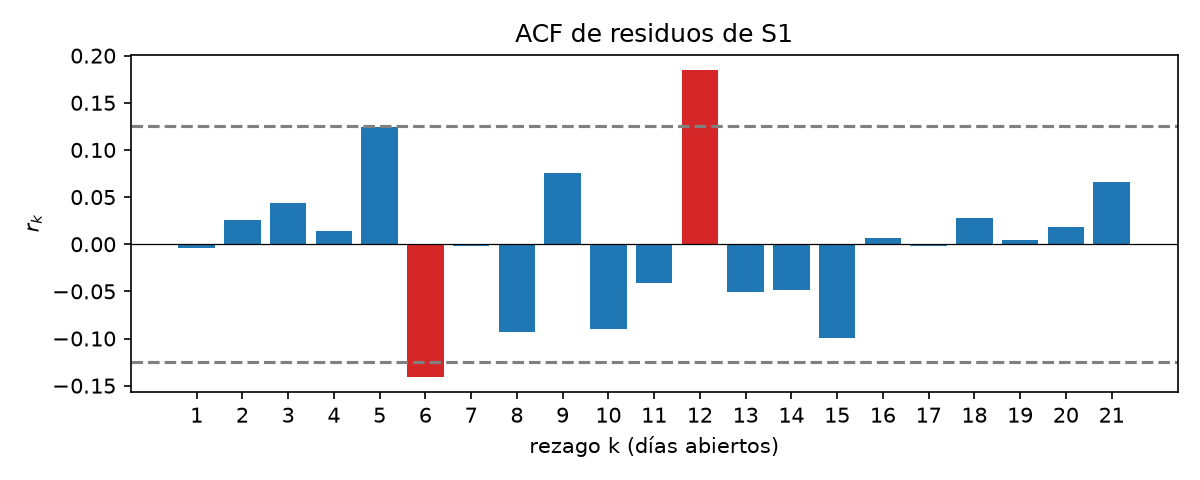
\includegraphics[width=0.48\textwidth]{p4_acf_s1.png}\hfill
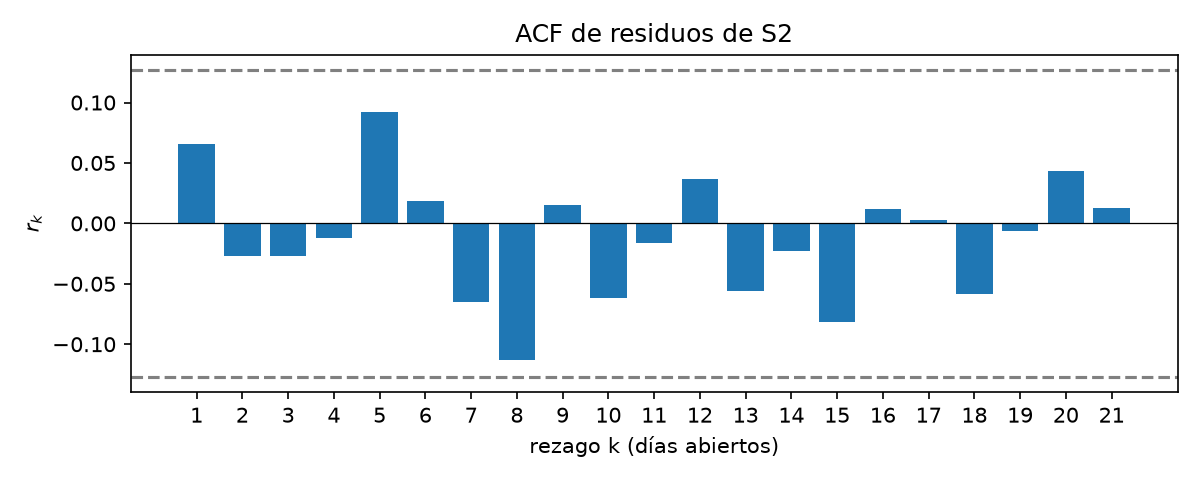
\includegraphics[width=0.48\textwidth]{p4_acf_s2.png}
\caption{ACF de los residuos de S1 (izquierda) y S2 (derecha).}
\end{figure}

\subsection*{4.5 Pronósticos a horizonte largo}
S1 es estacionario: como el AR(1), su pronóstico regresa a la media de forma exponencial. Con el horizonte creciendo se olvida del último valor y del patrón semanal (que decae como $0.52^{h/6}$) y converge a $\exp(\hat\mu)$, con $\hat\mu = \hat c/[(1-\hat\phi)(1-\hat\Phi)]$; aquí $\exp(\hat\mu)\approx$ £24\,980, y el pronóstico a 60 días es £24\,999. S2 no es estacionario: como la caminata aleatoria, nunca olvida. Su pronóstico no regresa a ninguna media: repite el último patrón semanal sobre el último nivel, y como tiene una diferencia regular y una estacional, puede arrastrar una pendiente (desde el 30 de septiembre sigue subiendo, Figura~\ref{fig:p4h}). La incertidumbre de S2 crece sin límite con el horizonte; la de S1 se estabiliza en la varianza incondicional.

\begin{figure}[H]\centering
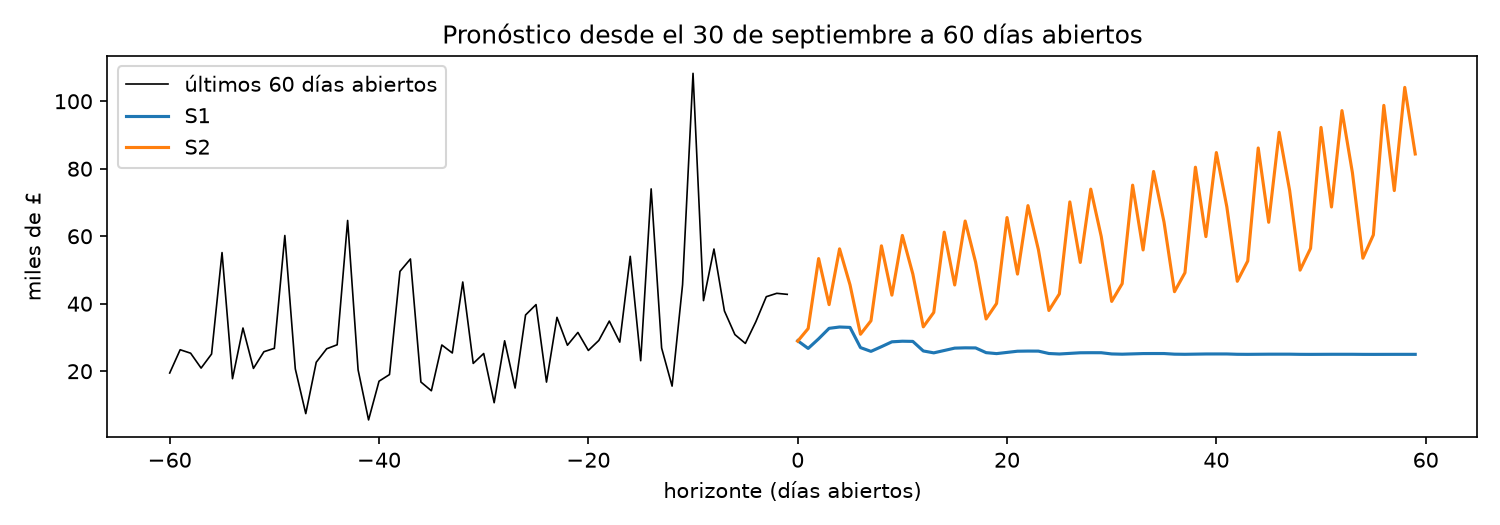
\includegraphics[width=0.85\textwidth]{p4_horizonte.png}
\caption{Pronóstico de S1 y S2 a 60 días abiertos desde el final del entrenamiento.}\label{fig:p4h}
\end{figure}

%======================================================================
\section{Parte 5: Pronóstico y fuga}

\subsection*{5.1 Modelos}
B1 (media histórica), B2 (\emph{naive} estacional), M1 (OLS con tendencia lineal en días calendario e indicadoras), M2 (indicadoras más $y_{t-7}$ y $y_{t-14}$), S1 y S2 están en \texttt{parte5\_pronostico.py}. Todos reciben solo la historia hasta el domingo de origen.

M2 puede usar $y_{t-7}$ porque los objetivos son los días de lunes a domingo después del origen: para cualquiera de ellos, $t-7$ cae a más tardar en el domingo de origen, que ya se observó. Con $y_{t-1}$ eso solo funciona para el lunes; para el martes haría falta la venta del lunes, que todavía no existe. S1 usa el rezago 1 de todas formas porque pronostica de forma recursiva: el pronóstico del martes usa el \emph{pronóstico} del lunes en lugar del valor real.

En cada reajuste S1 se ajustó con \texttt{maxiter=500} y S2 con el valor por defecto (las configuraciones que convergieron en 4.3), y se revisó \texttt{mle\_retvals['converged']} en los 32 orígenes (22 de mayo a septiembre y 10 de octubre a diciembre). S2 convergió en todos. S1 convergió en 31; en el origen del 6 de noviembre L-BFGS se quedó atascado en la búsqueda de línea aun con 2\,000 iteraciones, así que en ese origen se reajustó con Nelder--Mead partiendo de esos parámetros, y ahí sí convergió con parámetros casi idénticos (la log-verosimilitud mejora en 0.0002).

\subsection*{5.2 Tres formas de estimar el error}
\begin{table}[H]\centering\small
\caption{MAE y RMSE en miles de libras. (a) validación cruzada aleatoria de 5 folds sobre el entrenamiento, media y desviación estándar sobre 10 semillas; (b) origen móvil semanal dentro del entrenamiento (orígenes del 1 de mayo al 25 de septiembre); (c) periodo de prueba con origen móvil semanal (orígenes del 2 de octubre al 4 de diciembre).}\label{tab:val}
\resizebox{\textwidth}{!}{\tabla{p5_validacion}}
\end{table}

(a) no tiene sentido para B2, S1 y S2 porque esos modelos se definen por el orden del tiempo: B2 es ``el último valor del mismo día'', y S1 y S2 son recursiones que necesitan la serie contigua. Si se mezclan los días al azar, ``el último'' ya no existe y el modelo se entrenaría con datos posteriores al día que pronostica.

(b) se acerca más a (c) que (a): para M2, (a) da 8.35k, (b) 9.22k y (c) 15.23k; para M1, 9.12k, 9.76k y 15.18k. Pero ninguna se acerca de verdad: las dos estimaciones del entrenamiento se quedan cortas por 5 a 12 mil libras. La desviación estándar entre semillas en (a) es de apenas 50 a 190 libras, así que la diferencia no es ruido de la partición.

\subsection*{5.3 ¿Quién gana en prueba?}
Gana S2, con MAE de £12\,355 y RMSE de £15\,696, seguido de B2 (£14\,147 y £18\,374). En el entrenamiento (b) S2 no era el mejor (M2 tenía menor error), pero el periodo de prueba es distinto: es la temporada alta, con un nivel que sube semana a semana (Figura~\ref{fig:p5}). Los modelos que promedian la historia (B1, M1 con su tendencia lineal de todo el año, M2 con medias por día fijas, S1 que regresa a su media) se quedan abajo en noviembre. S2, con sus dos diferencias, se reajusta al nivel de la última semana igual que B2, pero promediando el ruido con sus términos MA en lugar de copiar una sola semana. Eso es consistente con 4.4: S2 era el único con residuos de ruido blanco, es decir, el único que ya había capturado el nivel que se mueve.

\begin{figure}[H]\centering
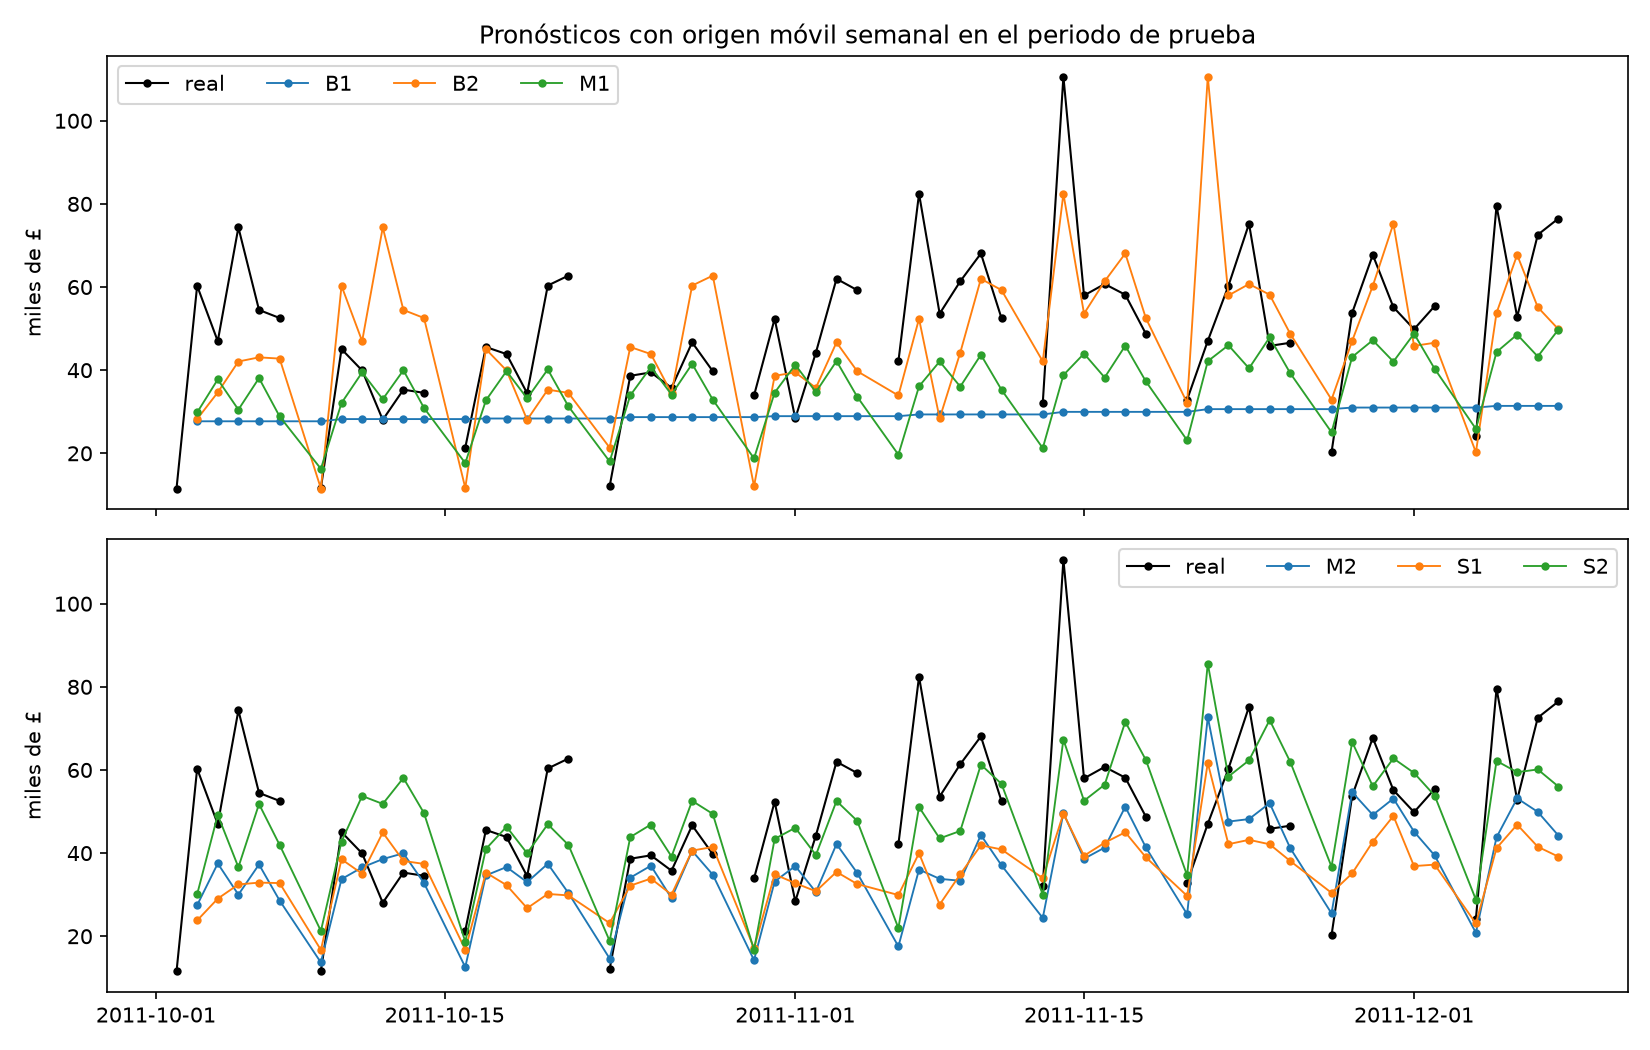
\includegraphics[width=\textwidth]{p5_prueba.png}
\caption{Pronósticos con origen móvil contra la venta real de octubre a diciembre.}\label{fig:p5}
\end{figure}

\subsection*{5.4 La trampa}
\begin{table}[H]\centering\small
\caption{M2 con y sin la media móvil centrada de 7 días como predictor (miles de £).}
\tabla{p5_trampa}
\end{table}

Con la media móvil se ve mejor: el MAE baja de 8.35k a 7.43k en (a) y de 9.22k a 8.24k en (b). Pero el predictor es ilegal. La media móvil centrada en $t$ es $(y_{t-3}+\dots+y_{t+3})/7$: contiene la propia venta que se quiere pronosticar y tres días del futuro. El origen móvil no lo detecta porque solo controla qué \emph{filas} se usan para ajustar; si la columna de la media móvil se calculó una sola vez sobre toda la serie, cada fila ya trae información del futuro adentro, aunque la fila se use en el momento correcto. Y (c) no se puede calcular sin trampa porque, parado en el domingo de origen, la media móvil del jueves siguiente necesita las ventas hasta el domingo próximo, que todavía no existen. Habría que pronosticarlas primero, y entonces ya no es la misma variable.

\subsection*{5.5 ¿Por qué se quedan cortas?}
Hay dos causas. La primera es cómo se partieron los datos: la validación cruzada aleatoria evalúa interpolación (el modelo ve días antes y después del que pronostica) y no extrapolación, y los vecinos se parecen. Esa se arregla con mejor validación, y por eso (b) se acerca más a (c) que (a). La segunda es que la serie cambió: octubre a diciembre es la temporada navideña, con un nivel y una volatilidad que no aparecen en ninguna parte del entrenamiento usado en (b). Ninguna validación dentro del entrenamiento puede ver algo que no está en los datos, así que esa no se arregla validando mejor. Con un solo año de datos no se puede estimar la estacionalidad anual: tenemos una sola temporada navideña (y ni siquiera completa al inicio), así que no hay forma de distinguir ``cada año sube en noviembre'' de ``este año la tendencia subió''. Haría falta al menos dos o tres años.

%======================================================================
\section{Parte 6: Análisis RFM}

\subsection*{6.1 R, F y M}
Con los datos limpios con \texttt{CustomerID} y solo transacciones antes del 1 de octubre de 2011: la recencia es el número de días entre la última factura de venta y el 1 de octubre, la frecuencia es el número de facturas de venta distintas (sin contar cancelaciones) y el monto es la venta neta (con las cancelaciones restando). Hay 3\,613 clientes con al menos una factura de venta. Otros 35 solo tienen cancelaciones antes del corte (de compras que no aparecen en los datos); no tienen ninguna compra, así que no tienen recencia y no entran al RFM.

Hay 7 clientes con $M\le0$: cuatro con $M=0$ (por ejemplo, el 12346 de los frascos de 1.4, que compró y canceló todo) y tres con $M$ negativo, que cancelaron más de lo que compraron dentro del periodo. Se dejan en el análisis, como pide 6.2, y les toca el puntaje más bajo en $M$, que es lo que corresponde a un cliente que no le dejó dinero a la tienda.

No se puede usar nada posterior al 1 de octubre porque la pregunta de 6.3 es si el cliente compra entre el 1 de octubre y el 8 de diciembre. Si la recencia o la frecuencia incluyeran esas compras, la variable que queremos predecir estaría dentro de los predictores (la misma fuga que la trampa de 5.4): un cliente que compró en noviembre tendría recencia baja \emph{porque} compró.

\subsection*{6.2 Puntajes}
El problema es F: el 40.2\,\% de los clientes tiene $F=1$ y solo hay 47 valores distintos. Los quintiles necesitan cortes en el 20\,\%, 40\,\%, etc., y con tantos empates no se puede cortar sin partir un grupo de clientes idénticos. Con el desempate al azar (orden por \texttt{CustomerID}, permutación con \texttt{default\_rng(2026)} y \texttt{rank(method='first')}) quedan cinco grupos de 722--723 clientes:

\begin{table}[H]\centering\small
\caption{Rango de F dentro de cada puntaje.}
\tabla{p6_rangos_f}
\end{table}

Los puntajes 1 y 2 tienen exactamente los mismos clientes ($F=1$), y el 3 también incluye clientes con $F=1$. Para dos clientes con la misma F que caen en puntajes distintos, la diferencia no dice nada: es puro azar de la permutación. Cualquier conclusión que distinga el puntaje 1 del 2 en F no tiene sentido.

\subsection*{6.3 ¿Quién vuelve a comprar?}
\begin{table}[H]\centering\small
\caption{Fracción de clientes que compró entre el 1 de octubre y el 8 de diciembre, por puntaje. La tasa base es 0.508.}
\tabla{p6_fraccion_compra}
\end{table}

\begin{figure}[H]\centering
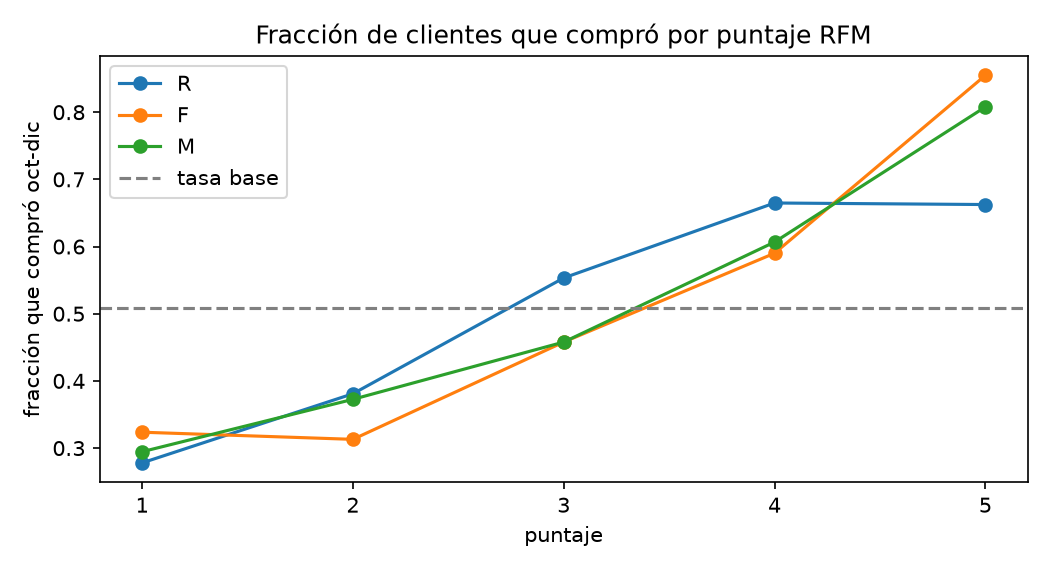
\includegraphics[width=0.65\textwidth]{p6_fraccion_compra.png}
\caption{Fracción que compró por puntaje en cada dimensión.}
\end{figure}

La que mejor separa es F: va de 0.32 en el puntaje 1 a 0.86 en el 5. M es parecida (0.30 a 0.81). R separa bien abajo pero se satura: los puntajes 4 y 5 compran casi igual (0.665 y 0.663). Como era de esperar, en F los puntajes 1 y 2 son iguales (0.32 y 0.31), porque son los mismos clientes con $F=1$ repartidos al azar.

\begin{table}[H]\centering\small
\caption{AUC de cada variable como clasificador de compra$_i$ (R con el signo invertido).}
\tabla{p6_auc}
\end{table}

Los AUC confirman el orden: F (0.720) $>$ M (0.709) $>$ R (0.673), y la suma de los tres puntajes es la mejor (0.734), aunque mejora poco sobre F sola porque las tres dimensiones están correlacionadas.

\subsection*{6.4 Campeones}
Los campeones (4 o 5 en las tres dimensiones) son 781 clientes, el 21.6\,\% de los clientes del RFM, y generaron el 53.2\,\% de la venta neta del 1 de octubre al 8 de diciembre de todos los clientes con \texttt{CustomerID} (£2.40 millones en total). Una quinta parte de los clientes deja más de la mitad de la venta.

\subsection*{6.5 Clientes nuevos}
723 clientes que compraron entre el 1 de octubre y el 8 de diciembre no tenían ninguna factura de venta antes del 1 de octubre, y generaron el 15.8\,\% de la venta neta de ese periodo. Un análisis RFM, o cualquier modelo construido cliente por cliente, no puede pronosticar esa venta: esos clientes no existen en la tabla, no tienen R, F ni M. Un modelo \emph{bottom-up} (pronosticar cada cliente y sumar) se quedaría corto en ese 16\,\% como mínimo. En cambio, el pronóstico de la Parte 5 es \emph{top-down}: pronostica la serie agregada, y la serie ya incluye a los clientes nuevos de cada temporada, así que los ve aunque no sepa quiénes son. Para el Proyecto 1 esto significa que, al comparar el pronóstico cliente por cliente contra el agregado, hay que sumarle al bottom-up un término para los clientes nuevos; si no, va a perder por construcción, sobre todo en la temporada navideña, cuando llegan más clientes.

%======================================================================
\begin{thebibliography}{9}
\bibitem{chen} D. Chen. \emph{Online Retail} [conjunto de datos]. UCI Machine Learning Repository, 2015. \url{https://archive.ics.uci.edu/dataset/352/online+retail}
\bibitem{chen2} D. Chen, S. L. Sain y K. Guo. Data mining for the online retail industry: A case study of RFM model-based customer segmentation using data mining. \emph{Journal of Database Marketing \& Customer Strategy Management}, 19(3):197--208, 2012.
\bibitem{fpp2} R. J. Hyndman y G. Athanasopoulos. \emph{Forecasting: Principles and Practice}, 2a ed. OTexts, 2018. \url{https://otexts.com/fpp2/}
\bibitem{tsay} R. S. Tsay. \emph{Analysis of Financial Time Series}, 2a ed. Wiley, 2005.
\end{thebibliography}

\end{document}
